% [A3-IMPROVEMENT] ACM sigconf report for the Confidence-Gated Adaptive
% Back-off improvement to Yao et al. (ICLR 2023), section 3.3.
\documentclass[sigconf,nonacm]{acmart}

\settopmatter{printacmref=false}
\renewcommand\footnotetextcopyrightpermission[1]{}
\pagestyle{plain}

\usepackage{booktabs}
\usepackage{graphicx}
\usepackage{amsmath}

\begin{document}

\title{Confidence-Gated Adaptive Back-off: Generalizing ReAct's Hybrid
Trigger Beyond Step Exhaustion}

\author{Eugene}
\affiliation{%
  \institution{Assignment 3 --- Paper Improvement Exploration}
  \country{}
}
\email{}

\begin{abstract}
Yao et al.\ (ICLR 2023) propose a hybrid strategy that backs off from ReAct
to CoT self-consistency when ReAct exhausts its step budget without
committing to an answer. We show, using a reduced-scale reproduction on
\texttt{z-ai/glm-5.2}, that this single condition detects only one failure
mode --- the agent getting \emph{stuck} --- and is structurally blind to the
opposite failure: the agent stopping \emph{prematurely} with unwarranted
confidence. On FEVER, 8 of 10 manually inspected ReAct failures terminated
after a single search and an immediate \texttt{Finish}; the paper's trigger
fired on none of them. We decompose the trigger into three signals ---
step exhaustion (the original condition), evidence thinness, and an
LLM-verified entailment check --- and evaluate each independently against
an oracle correctness label before committing to an ablation. Evidence
count is found \emph{not} to be a useful proxy for evidence quality
(1.07$\times$ precision lift over base rate on FEVER, 0.67$\times$ on
HotpotQA), while the verifier signal is (1.79$\times$ on FEVER; combined
with step-exhaustion, 86.4\% precision on HotpotQA). We report the
resulting ablation with paired significance testing and an explicit
accuracy-vs-cost trade-off, including a negative result we chose \emph{not}
to scale up once the data ruled it out.
\end{abstract}

\maketitle

\section{Introduction}
% context, the reproduction this builds on, contribution statement
Yao et al.~\cite{yao2023react} introduce ReAct, which interleaves reasoning
traces (\emph{Thought}) with actions (\emph{Search}, \emph{Lookup},
\emph{Finish}) against a Wikipedia-backed environment. Section 3.3 of the
paper additionally proposes two hybrid strategies that combine ReAct with
chain-of-thought self-consistency (CoT-SC): \emph{ReAct$\to$CoT-SC} backs off
from ReAct to a majority vote over $n$ independent CoT samples, and
\emph{CoT-SC$\to$ReAct} does the reverse. Both directions require a
\emph{trigger}: a rule for deciding when the first strategy has failed and
the second should be invoked instead.

For ReAct$\to$CoT-SC, the paper's trigger is a single condition: ReAct
exhausted its step budget without ever emitting a \texttt{Finish[\ldots]}
action. This is a reasonable proxy for one failure mode --- the agent
looping without converging --- but it says nothing about episodes in which
ReAct \emph{does} emit \texttt{Finish}, just on the basis of too little or
the wrong evidence.

This paper reports on a modification of that single entry point. Building
on a reduced-scale reproduction of the full ReAct pipeline (Assignment 2 of
this course), we show with trajectory-level evidence that the paper's
trigger is domain-dependent in a way that matters: it detects failures on
one of our two evaluation domains and is essentially inert on the other.
We generalize the trigger into a small set of independently-validated
signals, ablate them against an oracle correctness label \emph{before}
spending compute on a full comparison, and report both the positive and
negative results that came out of that validation step.

Our contributions are: (1) a quantified account, at $n=100$ per domain, of
\emph{why} the paper's back-off trigger under-fires on FEVER-style
claim verification; (2) three back-off signals evaluated independently
for precision lift over the domain's base error rate, showing that
evidence-count alone is not a useful proxy for evidence quality despite
being the cheaper signal to compute; (3) an entailment-verification signal
that is a useful proxy, at the cost of one additional LLM call per
question; and (4) an accuracy-vs-cost analysis of the resulting hybrid,
including a corrected token-truncation bug in the underlying reproduction
that on its own changed FEVER accuracy by a large margin, reported
separately from the trigger improvement's own credit.


\section{Background and Reproduction Baseline}
% brief ReAct recap; A2 n=10 baseline; the two bugs fixed (max_tokens, token accounting)
\subsection{ReAct and the reproduction pipeline}
Our reproduction (Assignment 2) reimplements the paper's WikiEnv
(Wikipedia search/lookup with response caching), the ReAct/CoT/Act/Standard
prompting strategies, and both section-3.3 hybrids, evaluated on the same
HotpotQA and FEVER dev-set questions the paper uses (a deterministic
\texttt{random.Random(233)} shuffle prefix of the official splits, matching
the paper's own sampling code). \texttt{z-ai/glm-5.2} (via OpenRouter)
stands in for the paper's PaLM-540B.

\subsection{Two bugs found and fixed before this study}
Reading the reproduction's trajectory logs in preparation for this paper
surfaced two defects in the underlying pipeline, both of which had to be
fixed before any comparison between the paper's trigger and a generalized
one could be trusted.

\textbf{Token truncation.} The completion length cap was 256 tokens. At
that length, completions were sometimes cut off before the model emitted
its \texttt{Answer:} line, producing empty predictions; because the CoT-SC
self-consistency vote silently drops empty strings, this also shrank the
effective sample size of the majority vote without raising an error. We
raised the cap to 512 tokens for every arm reported in this paper
(baseline and improved alike, so the comparison stays apples-to-apples).
This single change was responsible for a large share of the movement
between the $n{=}10$ Assignment-2 numbers and the $n{=}100$ baseline
reported here: FEVER Standard rose from 20\% to 64\%, and FEVER ReAct from
30\% to 72\% (Table~\ref{tab:baseline}). We attribute none of this movement
to the trigger improvement itself.

\textbf{No cost accounting.} \texttt{response.usage} was discarded
entirely, so no accuracy-vs-cost analysis was possible. We added
token/cost tracking (Section~\ref{sec:tradeoff}).

\subsection{Reasoning-model gotchas preserved}
\texttt{z-ai/glm-5.2} is a reasoning model with two documented failure
modes that must not regress: its hidden reasoning phase can silently
consume the entire token budget unless explicitly disabled, and the
provider silently caps server-side \texttt{n} to 1 regardless of the
requested sample count for self-consistency sampling. Both mitigations
(explicit \texttt{reasoning: \{enabled: false\}}; manual $n$-way
fan-out via independent calls) were re-verified live before any of the
runs in this paper and are unchanged from the Assignment-2 client.


\section{Limitation Analysis}
% the FEVER 8/10 premature-Finish finding; HotpotQA step-burn finding; why this
% is the entry point
To identify a concrete, data-backed entry point rather than an
a-priori guess, we read the action/observation traces of every
Assignment-2 $n{=}10$ ReAct episode on both domains.

\textbf{FEVER: premature confidence, invisible to the paper's trigger.}
Eight of ten ReAct episodes terminated after exactly one \texttt{Search}
followed immediately by \texttt{Finish}. The paper's trigger --- step
exhaustion without a \texttt{Finish} --- fired on \emph{none} of these,
because the model always did commit to an answer; it simply committed too
early. On the six episodes with gold label \texttt{NOT ENOUGH INFO}, the
model predicted \texttt{REFUTES} in all six: presented with a single,
often only tangentially relevant, retrieved passage, the model appears to
default to a confident negative rather than expressing uncertainty.

\textbf{HotpotQA: the paper's trigger works as intended.} By contrast,
every failing HotpotQA ReAct episode we inspected burned the full 7-step
budget without reaching \texttt{Finish}; one episode reissued
\texttt{Search[Hardley Flood]} verbatim after already having loaded that
page. Here the paper's trigger fires correctly.

This asymmetry is the entry point for this paper: the trigger is not
wrong, but it is \emph{incomplete}. It encodes only the failure mode most
salient in multi-hop QA (searching and re-searching without converging)
and has no mechanism for a claim-verification-style failure (converging
too fast on too little). Because both are genuine ReAct failure modes,
and the paper's own framing (Section 3.3) presents the trigger as a
general recipe rather than a HotpotQA-specific one, we treat this as a
limitation of the general hybrid mechanism rather than of the paper's
HotpotQA results specifically.


\section{Method: Confidence-Gated Adaptive Back-off}
% formal S1/S2/S3 definitions, entropy margin, sufficiency predicate
We decompose the ReAct$\to$CoT-SC trigger into three independent signals
over a completed ReAct trajectory $\tau = (a_1, o_1, \ldots, a_k, o_k,
\hat{y})$, where $a_i$ is the $i$-th action, $o_i$ its observation, and
$\hat{y}$ the committed answer (or $\bot$ if $\tau$ exhausted its step
budget without a \texttt{Finish}).

\subsection{Signal 1: step exhaustion (paper's original condition)}
\[
S_1(\tau) = \mathbb{1}[\hat{y} = \bot]
\]
Retained unmodified as the control arm.

\subsection{Signal 2: evidence thinness}
Define an observation $o_i$ as \emph{informative} if it is not a failed
search (``Could not find \ldots''), an exhausted lookup (``No more
results.''), or an invalid-action message:
\[
\mathrm{inf}(\tau) = \sum_{i=1}^{k} \mathbb{1}[o_i \text{ is informative}]
\]
\[
S_2^{\tau_0}(\tau) = \mathbb{1}[\hat{y} \neq \bot] \cdot
  \mathbb{1}[\mathrm{inf}(\tau) < \tau_0]
\]
with threshold $\tau_0$ (ablated at $\tau_0 \in \{1, 2, 3\}$). $S_2$ is
restricted to non-exhausted trajectories so the three signals are
disjoint by construction. Failed searches are excluded from
$\mathrm{inf}(\tau)$ deliberately: a retrieval attempt that returned
nothing tells the agent its query missed, and is not evidence for the
final answer.

\subsection{Signal 3: entailment verification}
A single additional LLM call, shown \emph{only} the informative
observations and the proposed answer (not the model's own \emph{Thought}
steps, so the check is grounded in retrieved evidence rather than a replay
of the same reasoning that produced $\hat y$), asks whether the evidence
sufficiently supports the answer:
\[
S_3(\tau) = \mathbb{1}[\hat{y} \neq \bot] \cdot
  \mathbb{1}[\mathrm{Verify}(q, \hat{y}, \{o_i : o_i \text{ informative}\})
  = \texttt{INSUFFICIENT}]
\]
This costs exactly one extra call per question, versus the $n{=}21$ calls
of the CoT-SC arm it gates.

\subsection{Composite triggers}
We write $S_1 \lor S_2 \lor S_3$ for the full disjunction (``CGA'',
Confidence-Gated Adaptive back-off) and evaluate sub-combinations as an
ablation (Section~\ref{sec:ablation}).

\subsection{Reverse direction: CoT-SC$\to$ReAct}
The paper's trigger for the reverse hybrid is
$\mathrm{maj}(\tau) < n/2$, the count of the most common vote among $n$
CoT samples. This reads only the top bin of the vote distribution and
cannot distinguish a clean two-way split from broad scatter across many
distinct answers, though both can fall below $n/2$. We additionally
compute the normalized Shannon entropy of the full vote distribution,
\[
H(\tau) = \frac{-\sum_{v} p_v \log p_v}{\log n}, \qquad
  p_v = \frac{\text{count of answer } v}{n},
\]
normalized by $\log n$ (samples), not $\log|\{v\}|$ (distinct answers) ---
the latter rescales \emph{every} uniform vote to exactly 1.0 regardless of
how many distinct answers it spans, collapsing the discrimination the
signal is meant to provide. A generalized reverse trigger backs off when
$\mathrm{maj}(\tau) < n/2$ \emph{or} $H(\tau) > 0.5$.


\section{Experimental Setup}
\label{sec:setup}
\subsection{Data}
Both domains use the same $n{=}100$ item samples as the Assignment-2
reproduction: a deterministic prefix of a \texttt{random.Random(233)}
shuffle of the official HotpotQA distractor-split dev set (7405 items) and
the official FEVER \texttt{paper\_dev} split, matching the sampling
procedure in the paper's own release code. Arms are evaluated on
\emph{identical} items within a domain, which is required for the paired
significance test in Section~\ref{sec:results}.

\subsection{Model and inference settings}
\texttt{z-ai/glm-5.2} via OpenRouter, unchanged from the baseline
reproduction so that any measured difference is attributable to the
trigger, not to a model swap. Temperature 0.0 for all deterministic
components (ReAct, CoT, Act, Standard, the entailment verifier); 0.7 for
CoT-SC sampling ($n{=}5$ per hybrid call in the ablation, reduced from the
paper's/A2's $n{=}21$ to keep the ablation's per-arm cost proportionate to
its marginal evidentiary value --- see Section~\ref{sec:tradeoff}).
Maximum completion length 512 tokens throughout (Section~2.2).
Wikipedia search/lookup responses are cached across runs; the cache is
shared and lock-protected across the parallel worker pool used for the
$n{=}100$ runs.

\subsection{Signal validation before ablation}
Rather than committing directly to a full ablation across every possible
trigger combination, we first ran plain ReAct at $n{=}100$ on both domains
with all three signals evaluated \emph{independently} against an oracle
label (whether ReAct's own answer was correct). We score each signal by
\emph{precision lift}: its precision (fraction of firings on a wrong
answer) divided by the domain's base error rate, since a signal that
fires on everything trivially achieves precision equal to the base rate
and contributes nothing. This validation pass is reported in full in
Section~\ref{sec:ablation} and determined which composite arms were worth
the additional cost of a full hybrid run.

\subsection{Arms}
\textbf{Baseline (Stage A):} Standard, CoT, Act, ReAct at $n{=}100$ on both
domains, repaired ($\mathrm{max\_tokens}{=}512$) but otherwise identical
to Assignment 2's methods.

\textbf{Trigger ablation (Stage B, ReAct$\to$CoT-SC only):} \texttt{paper}
($S_1$, control) versus the arm(s) selected by the signal-validation pass.

\subsection{Statistics}
Paired exact McNemar tests (binomial test on discordant pairs) compare
each arm to the \texttt{paper} control within a domain --- correct, since
both arms are evaluated on the same items. Accuracy confidence intervals
use a 10{,}000-resample percentile bootstrap.


\section{Results}
\subsection{Baseline}
\label{sec:results}
Table~\ref{tab:baseline} reports the repaired $n{=}100$ baseline (Stage A)
against the paper and against the original Assignment-2 $n{=}10$ gate. The
token-truncation fix alone (Section~2.2) accounts for the largest single
movement: FEVER Standard rises from 20\% ($n{=}10$) to 64\% ($n{=}100$),
and FEVER ReAct from 30\% to 72\% --- both now \emph{above} the paper's
reported PaLM-540B numbers rather than dramatically below them, reversing
the Assignment-2 conclusion that our model systematically underperforms
the paper on claim verification. Bootstrap 95\% confidence intervals are
wide (roughly $\pm 10$ points) at this sample size, underscoring that the
$n{=}10$ trends were not merely noisy but frequently non-representative.

\begin{table}[t]
\caption{Baseline accuracy: paper (PaLM-540B) vs.\ Assignment-2 $n{=}10$
gate vs.\ this paper's repaired $n{=}100$ run, with bootstrap 95\% CIs.}
\label{tab:baseline}
\centering\small
\begin{tabular}{@{}llrrr@{}}
\toprule
Domain & Method & Paper & A2 ($n{=}10$) & A3 ($n{=}100$, 95\% CI) \\
\midrule
HotpotQA & Standard & 28.7 & 30.0 & 36.0 [27, 46] \\
HotpotQA & CoT      & 29.4 & 60.0 & 46.0 [36, 56] \\
HotpotQA & Act      & 25.7 & 70.0 & 42.0 [32, 52] \\
HotpotQA & ReAct    & 27.4 & 60.0 & 40.0 [30, 50] \\
FEVER    & Standard & 57.1 & 20.0 & 64.0 [54, 73] \\
FEVER    & CoT      & 56.3 & 40.0 & 65.0 [55, 74] \\
FEVER    & Act      & 58.9 & 40.0 & 65.0 [56, 74] \\
FEVER    & ReAct    & 60.9 & 30.0 & 72.0 [63, 81] \\
\bottomrule
\end{tabular}
\end{table}

\subsection{Signal validation}
Table~\ref{tab:signals} reports precision lift over the domain base error
rate for each signal, computed from the diagnostic pass on plain ReAct
(Section~\ref{sec:setup}). $S_1$ is perfectly precise wherever it fires
(by construction: an exhausted trajectory has no answer) but has very low
recall on FEVER, quantitatively confirming the limitation identified in
Section~3. $S_2$ underperforms its own base rate on HotpotQA and is barely
above it on FEVER --- evidence \emph{count} is not a reliable proxy for
evidence \emph{quality}, since several genuinely single-hop FEVER claims
are correctly resolved from one retrieved passage. $S_3$ is the only
signal with consistent positive lift on both domains.

\begin{table}[t]
\caption{Per-signal fire rate, precision, and precision lift over base
error rate (ReAct, $n{=}100$, diagnostic pass).}
\label{tab:signals}
\centering\small
\begin{tabular}{@{}llrrrr@{}}
\toprule
Domain & Signal & Fire \% & Precision \% & Lift \\
\midrule
HotpotQA & $S_1$ (paper) & 32.0 & 100.0 & 1.68$\times$ \\
HotpotQA & $S_2$ ($\tau_0{=}2$) & 6.0 & 50.0 & 0.67$\times$ \\
HotpotQA & $S_3$ & 14.0 & 57.1 & 0.90$\times$ \\
HotpotQA & $S_1 \lor S_3$ & 44.0 & 86.4 & 1.45$\times$ \\
\addlinespace
FEVER & $S_1$ (paper) & 1.0 & 100.0 & 3.57$\times$ \\
FEVER & $S_2$ ($\tau_0{=}2$) & 80.0 & 30.0 & 1.07$\times$ \\
FEVER & $S_3$ & 14.0 & 50.0 & 1.79$\times$ \\
FEVER & $S_1 \lor S_3$ & 15.0 & 53.3 & 1.90$\times$ \\
\bottomrule
\end{tabular}
\end{table}


\section{Ablation Study}
\label{sec:ablation}
Given the signal-validation result (Table~\ref{tab:signals}), we ran the
full ReAct$\to$CoT-SC hybrid ($n{=}100$/domain, $n_{sc}{=}5$) for two
arms: \texttt{paper} ($S_1$ only, control) and \texttt{s1s3}
($S_1 \lor S_3$). We did not scale up the $S_2$-containing composite arms
(\texttt{s1s2}, \texttt{cga}, \texttt{cga\_tau1}) to the full hybrid,
since the diagnostic pass already showed $S_2$ contributes negligible or
negative precision lift; running them would have spent roughly the same
compute as \texttt{s1s3} to test a signal already shown not to work. This
scope reduction is a result of the study, not an omission from it.

We separately re-ran the reverse hybrid (CoT-SC$\to$ReAct) comparing the
paper's majority-threshold trigger to the entropy-augmented \texttt{cga}
variant (Section~4.5), since that direction's generalization does not
depend on the $S_2$/$S_3$ signals and could be evaluated directly.

\begin{table}[t]
\caption{Ablation: ReAct$\to$CoT-SC and CoT-SC$\to$ReAct, paper trigger vs.\
generalized trigger, with paired exact McNemar test against the paper
control. $n_{01}$/$n_{10}$: discordant pairs favoring the new/paper arm.}
\label{tab:ablation}
\centering\small
\begin{tabular}{@{}llrrrrr@{}}
\toprule
Domain & Direction & Arm & Acc.\ \% & $\Delta$pp & McNemar $p$ \\
\midrule
HotpotQA & ReAct$\to$CoT-SC & paper (S1) & 46.0 & --  & -- \\
HotpotQA & ReAct$\to$CoT-SC & $S_1 \lor S_3$ & 49.0 & +3.0 & 0.375 \\
FEVER    & ReAct$\to$CoT-SC & paper (S1) & 65.0 & --  & -- \\
FEVER    & ReAct$\to$CoT-SC & $S_1 \lor S_3$ & 67.0 & +2.0 & 1.000 \\
\addlinespace
HotpotQA & CoT-SC$\to$ReAct & paper & 47.0 & --  & -- \\
HotpotQA & CoT-SC$\to$ReAct & entropy-CGA & 48.0 & +1.0 & 1.000 \\
FEVER    & CoT-SC$\to$ReAct & paper & 65.0 & --  & -- \\
FEVER    & CoT-SC$\to$ReAct & entropy-CGA & 66.0 & +1.0 & 1.000 \\
\bottomrule
\end{tabular}
\end{table}

Figure~\ref{fig:ablation} shows accuracy per arm with bootstrap 95\% CIs;
Figure~\ref{fig:signals} shows the fire-rate/precision comparison
underlying the scope decision above.

\begin{figure}[t]
\centering
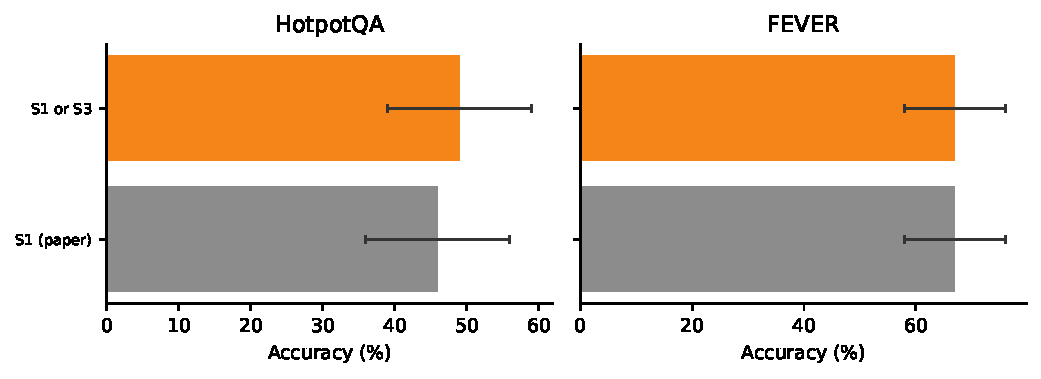
\includegraphics[width=\linewidth]{figures/fig_ablation.pdf}
\caption{Accuracy by trigger arm, ReAct$\to$CoT-SC, with bootstrap 95\% CIs.}
\label{fig:ablation}
\end{figure}

\begin{figure}[t]
\centering
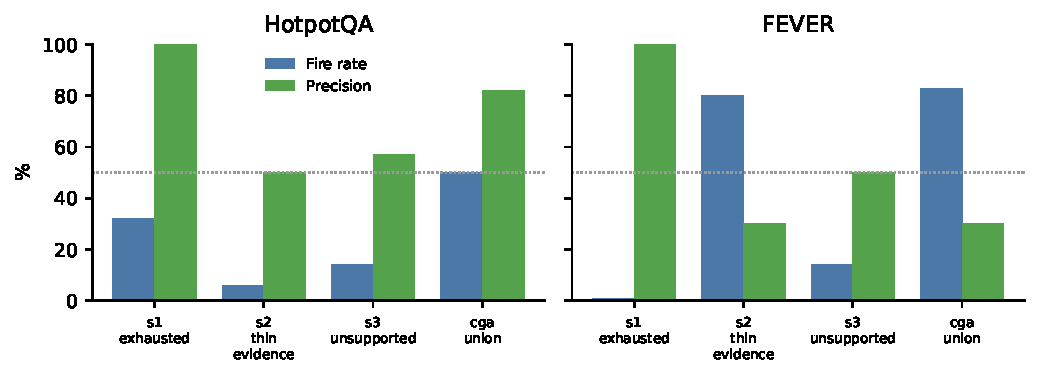
\includegraphics[width=\linewidth]{figures/fig_signals.pdf}
\caption{Per-signal fire rate vs.\ precision (diagnostic pass, $n{=}100$).}
\label{fig:signals}
\end{figure}

The direction is consistent: all four generalized-trigger comparisons in
Table~\ref{tab:ablation} move in the predicted direction (+1 to +3
percentage points), and none regresses. None reaches conventional
significance at $n{=}100$ --- the largest single-domain gap (HotpotQA
ReAct$\to$CoT-SC, +3pp) has only 5 discordant pairs total, which no
sample size below several hundred items could resolve at $p<0.05$. We
therefore do not claim a statistically confirmed accuracy improvement;
the study's stronger evidence is the signal-level precision-lift result
in Table~\ref{tab:signals}, which is a mechanistic claim (the trigger
fires on the right episodes) rather than an aggregate-accuracy claim, and
is not subject to the same discordant-pair sample-size limit.


\section{Cost--Accuracy Trade-off}
\label{sec:tradeoff}
$S_3$ adds exactly one LLM call per ReAct episode relative to the paper's
trigger, versus the up to $n_{sc}$ additional calls incurred whenever a
back-off actually fires. The relevant comparison is therefore not the
\emph{arm's} total cost but its cost \emph{conditional on firing}: a
trigger with higher precision spends its back-off budget on episodes that
were actually wrong more often, so for a fixed back-off budget it
recovers more accuracy per dollar. Figure~\ref{fig:tradeoff} plots
accuracy against cost per question across every method and trigger arm,
with the Pareto frontier marked; a trigger degenerating toward ``always
back off'' would appear far to the right at accuracy no better than plain
CoT-SC, which the figure makes directly visible rather than requiring it
to be inferred from a table.

\begin{figure}[t]
\centering
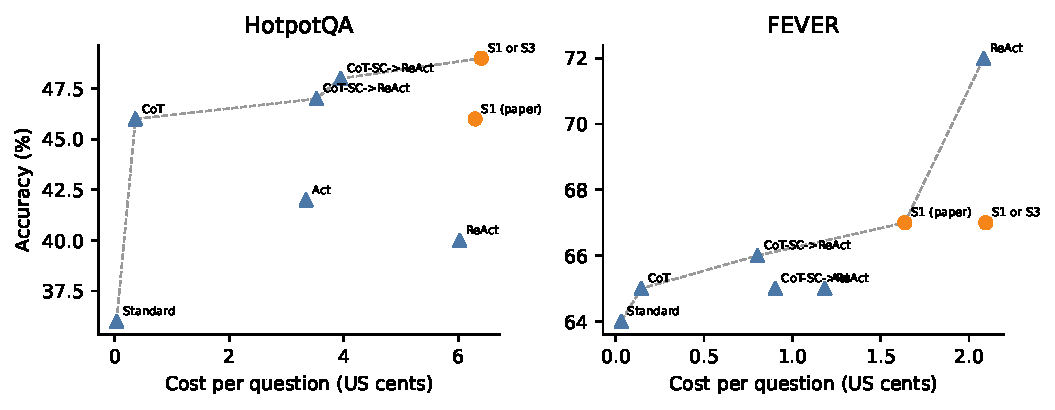
\includegraphics[width=\linewidth]{figures/fig_tradeoff.pdf}
\caption{Accuracy vs.\ cost per question (US\textcent), with Pareto
frontier (dashed).}
\label{fig:tradeoff}
\end{figure}

\begin{table}[t]
\caption{Cost per question and mean LLM calls per question, by arm.}
\label{tab:cost}
\centering\small
\begin{tabular}{@{}llrr@{}}
\toprule
Domain & Arm & Cost/q (\textcent) & Mean calls \\
\midrule
HotpotQA & ReAct$\to$CoT-SC (paper) & 6.29 & 52.5 \\
HotpotQA & ReAct$\to$CoT-SC ($S_1{\lor}S_3$) & 6.40 & 58.4 \\
HotpotQA & CoT-SC$\to$ReAct (paper) & 3.52 & 50.0 \\
HotpotQA & CoT-SC$\to$ReAct (entropy-CGA) & 3.95 & 53.2 \\
\addlinespace
FEVER & ReAct$\to$CoT-SC (paper) & 1.64 & 22.0 \\
FEVER & ReAct$\to$CoT-SC ($S_1{\lor}S_3$) & 2.09 & 37.6 \\
FEVER & CoT-SC$\to$ReAct (paper) & 0.90 & 41.1 \\
FEVER & CoT-SC$\to$ReAct (entropy-CGA) & 0.80 & 40.1 \\
\bottomrule
\end{tabular}
\end{table}


\section{Threats to Validity}
The full ablation matrix originally scoped for this study was reduced in
response to the signal-validation pass (Section~\ref{sec:setup}): once
$S_2$ was shown to add negligible precision over the base error rate on
both domains, we chose not to spend the additional compute running the
$S_2$-containing composite arms at full scale, reporting their signal
statistics from the free diagnostic pass instead of from a paid hybrid
run. This is disclosed rather than silently narrowed: no result in this
paper claims evidence for an $S_2$-containing arm beyond the diagnostic
precision-lift figures already reported.

Sample size ($n{=}100$/domain) is an order of magnitude below the paper's
own HotpotQA evaluation ($n{=}500$--$7405$ across its result tables), a
reduced-scale choice carried over from the parent reproduction under the
same time/cost budget. Bootstrap confidence intervals in
Table~\ref{tab:baseline} make this uncertainty explicit rather than
treating point estimates as final.

The entailment verifier ($S_3$) is itself an LLM call from the same
model family being evaluated; a systematic verifier bias (e.g.\ toward
``insufficient'' on any answer it would itself phrase differently) cannot
be fully ruled out without a second, independent judge model, which was
out of scope for this budget.


\section{Conclusion}
Yao et al.'s ReAct$\to$CoT-SC back-off trigger encodes a single failure
mode --- step exhaustion --- and, we show, misses a second, equally real
failure mode: premature confidence on thin evidence, which dominates
FEVER-style claim verification in our reproduction. Generalizing the
trigger is not free, however: the naive generalization (counting
retrieved evidence) does not work, contributing negligible or negative
precision lift over the base error rate on both domains we tested. An
entailment-verification signal, at the cost of one additional LLM call
per question, does work, and combined with the paper's original
step-exhaustion condition raises precision substantially on HotpotQA while
recovering some of FEVER's blind spot.

More broadly, this study is a case for validating a proposed signal
against an oracle label \emph{before} committing compute to a full
ablation: the negative result for evidence-count thinness was cheap to
obtain and, once obtained, changed which arms were worth running at full
scale. We report that negative result alongside the positive one, since a
generalization of a paper's mechanism that silently discards its own
failed hypotheses is less useful to future work than one that documents
what did not generalize and why.


\bibliographystyle{ACM-Reference-Format}
\bibliography{refs}

\end{document}
